\documentclass[11pt]{report}
\usepackage[utf8]{inputenc}
% \usepackage[landscape]{geometry}
\usepackage{graphicx}
\title{IVR Assignment}
\author{Maksymilian Mozolewski \& Martin Lewis}
\date{November 2020}
\newcommand\scalemath[2]{\scalebox{#1}{\mbox{\ensuremath{\displaystyle #2}}}}
\usepackage{amsmath}
\usepackage[margin=0.5in]{geometry}
\usepackage{float}

\let\cos\relax
\let\sin\relax
% \DeclareMathOperator{\cos}{\mathit{C}}
% \DeclareMathOperator{\sin}{\mathit{S}}
\newcommand{\sin}[1]{\mathit{S}_{#1}}
\newcommand{\cos}[1]{\mathit{C}_{#1}}

\begin{document}

% \maketitle

\section*{Github}
Sections 3,4 - s1751752
Section 2 - s1824863

\noindent Link to the github repository:  https://github.com/martin-lewis/ivrassignment

\section*{2.1}

The first part of this section was straight forward calculating the position of the angles based of the sinusoidal positions. This achieved with rospy's get\_time() function and sin.
This was then published to the topics to get the robot moving.

The next section is getting the 3D coordinates from the 2 2D images. This was done initially with a naive system that assumed that the camera was always orthogonal,
which it isn't. This worked fine for most cases except the extreme cases where the robot arm would point directly into a camera. This was replaced by a more complex
system considering the cameras to be simple pinhole cameras and reversing the projection into the 2D image back into the 3D world coordinates. Then the position
of the object in both cameras is considered together to find the height.

Finally having got the 3D world coordinates then the angles had to be found. We tried a few different methods, optimisation, projections but finally settling for using trigonometry. Using atan2 to find the values of
joint 2 and 3. Joint 2 is found with atan on the y and z components of the vector between the blue and green blobs. Then the vector is rotated by the found angle
and then atan is run on the x and z components for joint3. This does however mean that the uncertainly and error in the angle of joint 2 is passed to joint3.

You can see the two example sections of an rqt\_plot graph from joints 2 and 3 in figures 1 and 2.
\begin{figure}[H]
    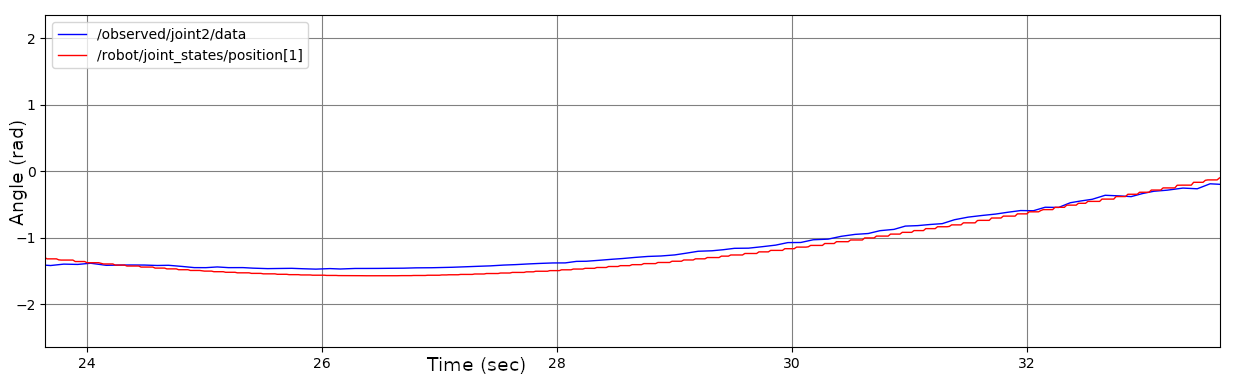
\includegraphics[width=\linewidth]{joint2.png}
    \caption{Joint2 Angle}
\end{figure}

\begin{figure}[H]
    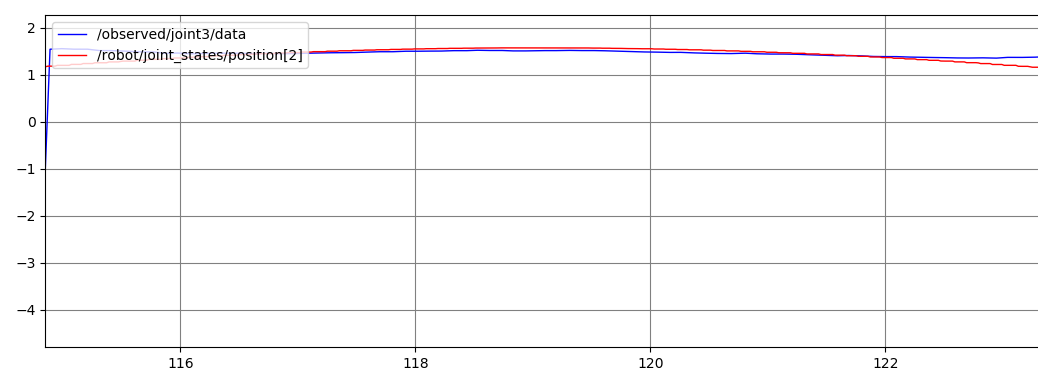
\includegraphics[width=\linewidth]{joint3.png}
    \caption{Joint3 Angle}
\end{figure}

Joint 4 however is calculated by a projection. This means its not reliant on the first two angles. It works out the angle between the vector between the
green and red blobs and the vector between the blue and green ones.

\begin{figure}
    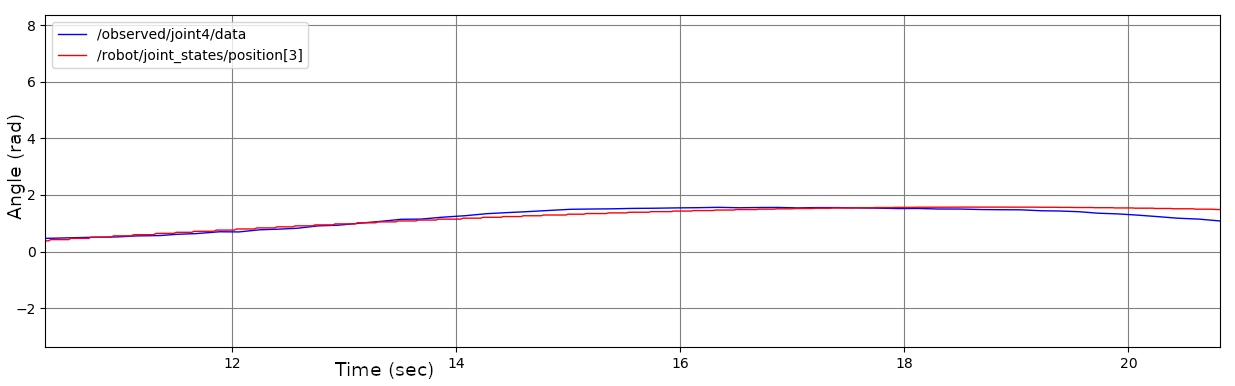
\includegraphics[width=\linewidth]{joint4.png}
    \caption{Joint4 Angle}
\end{figure}

\section*{2.2}

The target is distinguished first by a threshold over the colour orange. Then the cv2 match template function is applied to it using two templates
(template-box.png and template-sphere-png both are in root folder of the repository) this returns a position in the image supplied to it. This is then
turned into 3D world coordinates by the system discussed in 2.1. You can see a graph showing the results in figure 4. The major issue is that of the z value, it is 
frequently not quite correct, it usually in the correct ball park but not as accurate at the other two. X and Y however are very accurate for the vast majority of the time.

I suspect that the source of error comes mainly from the fact that the target is usually high up in the cameras view and that this means it's at more of an angle
reducing the accuracy of the algorithm in working out its Z coordinate.

\begin{figure}[H]
    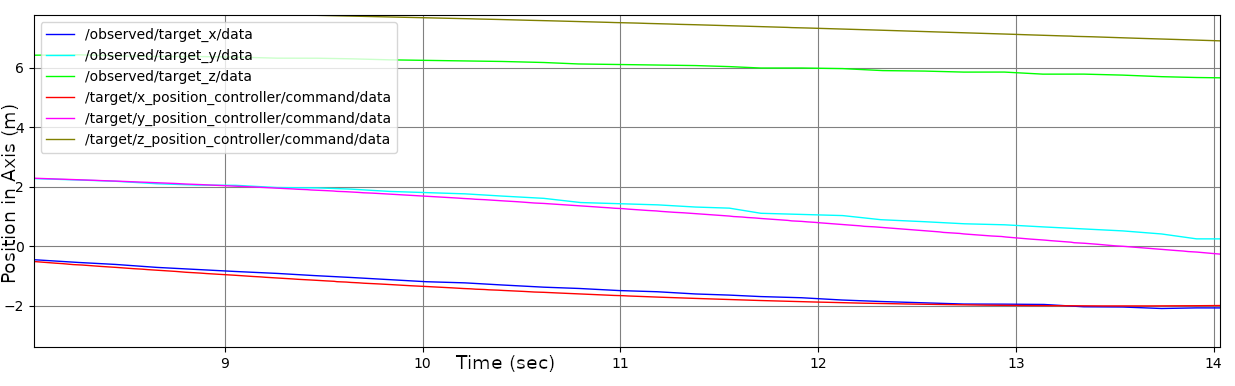
\includegraphics[width=\linewidth]{target.png}
    \caption{Target Position (/observed/...) and actual position (/target/...)}
\end{figure}

% ----------------- 3.1----------------- 

\section*{3.1 Forward Kinematics}
\subsection*{Presentation of the forward kinematics equation}

The final forward kinematics translation component looks like the following:\\


\begin{equation*}
FK(q) = 
\begin{bmatrix}
           x_{e} \\
           y_{e} \\
           z_{e}
\end{bmatrix} = 
\left(\begin{array}{c} %
    3 \left(\sin{q_{1}} \sin{q_{2}} \cos{q_{3}} + \sin{q_{3}} \cos{q_{1}}\right) \cos{q_{4}}  %
    + 3.5 \sin{q_{1}} \sin{q_{2}} \cos{q_{3}} %
    + 3 \sin{q_{1}} \sin{q_{4}} \cos{q_{2} } %
    + 3.5 \sin{q_{3}} \cos{q_{1}} %
    \\
    3 \left(\sin{q_{1}} \sin{q_{3}} %
    - \sin{q_{2}} \cos{q_{1}} \cos{q_{3}}\right) \cos{q_{4}} %
    + 3.5 \sin{q_{1}} \sin{q_{3}} %
    - 3.5 \sin{q_{2}} \cos{q_{1}} \cos{q_{3}} %
    - 3 \sin{q_{4}} \cos{q_{1}} \cos{q_{2}} %
    \\
    - 3 \sin{q_{2}} \sin{q_{4}} %
    + 3 \cos{q_{2}} \cos{q_{3}} \cos{q_{4}} %
    + 3.5 \cos{q_{2}} \cos{q_{3}} + 2.5
    \end{array}\right)
\end{equation*} \\


\subsection*{Comparing forward kinematics and vision algorithm's estimations of end-effector positions}

The robot was set to the different joint positions given in figure below. In the far column Euclidean distance is shown to compare the different estimations. We can see that all the estimations are between 0.5 and 0.75 meters off each other, this is quite close however not ideal. The highest differences appear for angles which direct the end effector closer or further to only one of the cameras, the source of error here is clearly not the forward kinematics equation, since those are the configurations which are the most problematic for vision. The sources of error here are:
\begin{itemize}
    \item Obfuscation of the end effector by the robot. Both partial and full obfuscation causes: a shift in the CoM of the blobs, and loss of accurate information respectively.
    \item Lighting variation, some of the blobs will sometimes be shifted very slightly when the colours become more shaded, this adds to the error and is likely the reason a constant error is present (this could be fixed by using the HSI colour space for thresholding instead)

\end{itemize}
\begin{figure}[h]

    \begin{center}
        \begin{tabular}{|c|c|c|c|c|c|c|}
        \hline 
         q1(rad)&q2(rad)&q3(rad)&q4(rad)&Vision EFPos &FK EFPos& Euclidian Distance(m) \\ \hline 
        0.50&-0.50&0.50&-0.50&[0.672 4.907 5.993]&[0.738 4.782 6.534]&0.56 \\ \hline 
        -0.50&0.50&-0.50&0.50&[-4.542 -2.081  5.983]&[-4.422 -1.962  6.534]&0.58 \\ \hline 
        0.50&0.50&0.50&0.50&[ 4.511 -2.067  5.977]&[ 4.422 -1.962  6.534]&0.57 \\ \hline 
        -0.50&-0.50&-0.50&-0.50&[-0.768  4.882  6.004]&[-0.738  4.782  6.534]&0.54 \\ \hline 
        1.00&0.50&-1.00&0.50&[-0.4   -6.1    4.117]&[-0.389 -5.883  4.718]&0.64 \\ \hline 
        0.50&1.00&-1.00&0.50&[-2.896 -5.787  2.423]&[-2.819 -5.603  3.08 ]&0.69 \\ \hline 
        1.57&1.57&0.10&0.10&[6.58  0.652 1.561]&[6.453 0.647 2.2  ]&0.65 \\ \hline 
        3.14&1.57&0.10&0.10&[-0.925  6.674  1.59 ]&[-0.647  6.453  2.2  ]&0.71 \\ \hline 
        -1.57&1.57&1.00&0.50&[-3.398 -5.339  0.359]&[-3.314 -5.161  1.062]&0.73 \\ \hline 
        -3.14&1.57&0.10&0.10&[-0.925  6.674  1.59 ]&[-0.647  6.453  2.2  ]&0.71 \\ \hline 
        \end{tabular}
    \end{center}
    \caption{The End Effector Position estimates at the different joint configurations (q1,q2,q3,q4) via FK and Vision}

\end{figure}


\section*{3.2 Closed-Loop Control}
\subsection*{Presentation of the velocity kinematics calculation}
The Jacobian was again calculated using SymPy to avoid errors, the resulting matrix is quite large and so we will present it split by columns:

\begin{equation*}
    
J(q)_{*,1} = 
\begin{bmatrix}
           \left(- 3 \sin{\left(q_{1} \right)} \sin{\left(q_{3} \right)} + 3 \sin{\left(q_{2} \right)} \cos{\left(q_{1} \right)} \cos{\left(q_{3} \right)}\right) \cos{\left(q_{4} \right)} - 3.5 \sin{\left(q_{1} \right)} \sin{\left(q_{3} \right)} + 3.5 \sin{\left(q_{2} \right)} \cos{\left(q_{1} \right)} \cos{\left(q_{3} \right)} + 3 \sin{\left(q_{4} \right)} \cos{\left(q_{1} \right)} \cos{\left(q_{2} \right)} \\
           
           \left(3 \sin{\left(q_{1} \right)} \sin{\left(q_{2} \right)} \cos{\left(q_{3} \right)} + 3 \sin{\left(q_{3} \right)} \cos{\left(q_{1} \right)}\right) \cos{\left(q_{4} \right)} + 3.5 \sin{\left(q_{1} \right)} \sin{\left(q_{2} \right)} \cos{\left(q_{3} \right)} + 3 \sin{\left(q_{1} \right)} \sin{\left(q_{4} \right)} \cos{\left(q_{2} \right)} + 3.5 \sin{\left(q_{3} \right)} \cos{\left(q_{1} \right)} \\
           
           0
\end{bmatrix} \\ \\

J(q)_{*,2} = 
\begin{bmatrix}
           - 3 \sin{\left(q_{1} \right)} \sin{\left(q_{2} \right)} \sin{\left(q_{4} \right)} + 3 \sin{\left(q_{1} \right)} \cos{\left(q_{2} \right)} \cos{\left(q_{3} \right)} \cos{\left(q_{4} \right)} + 3.5 \sin{\left(q_{1} \right)} \cos{\left(q_{2} \right)} \cos{\left(q_{3} \right)}
           \\
           3 \sin{\left(q_{2} \right)} \sin{\left(q_{4} \right)} \cos{\left(q_{1} \right)} - 3 \cos{\left(q_{1} \right)} \cos{\left(q_{2} \right)} \cos{\left(q_{3} \right)} \cos{\left(q_{4} \right)} - 3.5 \cos{\left(q_{1} \right)} \cos{\left(q_{2} \right)} \cos{\left(q_{3} \right)}
           \\
           - 3 \sin{\left(q_{2} \right)} \cos{\left(q_{3} \right)} \cos{\left(q_{4} \right)} - 3.5 \sin{\left(q_{2} \right)} \cos{\left(q_{3} \right)} - 3 \sin{\left(q_{4} \right)} \cos{\left(q_{2} \right)}
           
\end{bmatrix} \\ \\


J(q)_{*,3} = 
\begin{bmatrix}

 \left(- 3 \sin{\left(q_{1} \right)} \sin{\left(q_{2} \right)} \sin{\left(q_{3} \right)} + 3 \cos{\left(q_{1} \right)} \cos{\left(q_{3} \right)}\right) \cos{\left(q_{4} \right)} - 3.5 \sin{\left(q_{1} \right)} \sin{\left(q_{2} \right)} \sin{\left(q_{3} \right)} + 3.5 \cos{\left(q_{1} \right)} \cos{\left(q_{3} \right)}
 \\
 \left(3 \sin{\left(q_{1} \right)} \cos{\left(q_{3} \right)} + 3 \sin{\left(q_{2} \right)} \sin{\left(q_{3} \right)} \cos{\left(q_{1} \right)}\right) \cos{\left(q_{4} \right)} + 3.5 \sin{\left(q_{1} \right)} \cos{\left(q_{3} \right)} + 3.5 \sin{\left(q_{2} \right)} \sin{\left(q_{3} \right)} \cos{\left(q_{1} \right)}
 \\
 - 3 \sin{\left(q_{3} \right)} \cos{\left(q_{2} \right)} \cos{\left(q_{4} \right)} - 3.5 \sin{\left(q_{3} \right)} \cos{\left(q_{2} \right)}
 
 
\end{bmatrix}\\ \\

J(q)_{*,4} = 
\begin{bmatrix}
- \left(3 \sin{\left(q_{1} \right)} \sin{\left(q_{2} \right)} \cos{\left(q_{3} \right)} + 3 \sin{\left(q_{3} \right)} \cos{\left(q_{1} \right)}\right) \sin{\left(q_{4} \right)} + 3 \sin{\left(q_{1} \right)} \cos{\left(q_{2} \right)} \cos{\left(q_{4} \right)}
\\
- \left(3 \sin{\left(q_{1} \right)} \sin{\left(q_{3} \right)} - 3 \sin{\left(q_{2} \right)} \cos{\left(q_{1} \right)} \cos{\left(q_{3} \right)}\right) \sin{\left(q_{4} \right)} - 3 \cos{\left(q_{1} \right)} \cos{\left(q_{2} \right)} \cos{\left(q_{4} \right)}
\\
- 3 \sin{\left(q_{2} \right)} \cos{\left(q_{4} \right)} - 3 \sin{\left(q_{4} \right)} \cos{\left(q_{2} \right)} \cos{\left(q_{3} \right)}
\end{bmatrix}
\end{equation*} \\ \\

\noindent The algorithm deployed used the damped pseudo inverse of the Jacobian matrix. Only the Proportional and Derivative error components were used to direct the change in joint values at each iteration of the loop. 
The change in q (or angular velocity of q) at each iteration can be defined as follows: \\


\begin{equation*}
    \dot{q} = J^{\text{*}}(q) (K_{d} \dot{x}_{d} + K_{p}x_{\Delta} )
\end{equation*}

\noindent where $J^{\text{*}}_{d}(q) $ is the damped pseudo inverse defined as:
\begin{equation*}
    J^{\text{*}}(q) = J^{T}(JJ^{T} + \mathit{k}^{2}\mathbf{I})^{-1}
\end{equation*}\\

\noindent $x_{\Delta}$ is the difference between the desired and current end effector position.
\noindent $\dot{x}_{d}$ is the derivative of the end effector position and $K_{d}$,$K_{p}$ are the constants used to control the size of each step in relation to the derivative and proportional errors at each step respectively.

\subsection*{Evaluation of control loop}

\begin{figure}[H]

  \centering
  \begin{minipage}[b]{0.44\textwidth}
    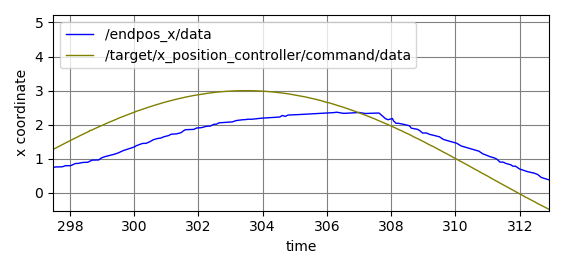
\includegraphics[width=\textwidth]{3.2.x.png}
    \caption{End effector x coordinate (/endpos/...) vs target sphere x coordinate (/target/...)}
  \end{minipage}
  \hfill
  \begin{minipage}[b]{0.44\textwidth}
    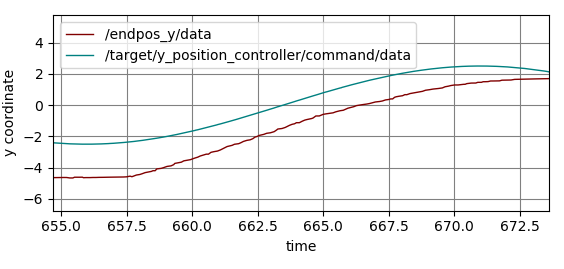
\includegraphics[width=\textwidth]{3.2.y.png}
    \caption{End effector y coordinate (/endpos/...) vs target sphere y coordinate (/target/...)}
  \end{minipage}
\begin{minipage}[b]{0.44\textwidth}
    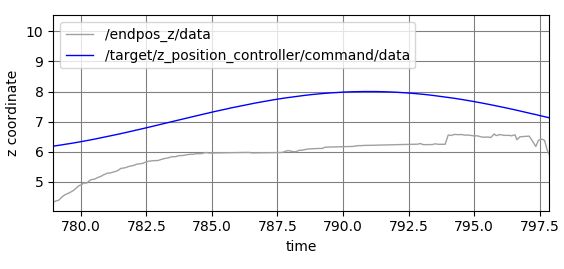
\includegraphics[width=\textwidth]{3.2.z.png}
    \caption{End effector z coordinate (/endpos/...) vs target sphere z coordinate (in world frame) (/target/...)}
  \end{minipage}
\end{figure}

\begin{figure}[h]
  \centering

\end{figure}

\section*{4.2 Null-space Control}
\subsection*{Algorithm}
The only amendment to the previous algorithm needed to allow for a secondary task maximisation, is the addition of the null-space projection term:
\begin{equation*}
    \dot{q} = J^{\text{*}}(q) (K_{d} \dot{x}_{d} + K_{p}x_{\Delta} ) + (\mathbf{I} - J^{\text{*}}J )\dot{q}_{0}
\end{equation*}

\noindent where $\dot{q}_{0}$ is the derivative of the "box" avoidance function w(q) defined as:
\begin{equation*}
    w(q) = || FK(q) - b ||
\end{equation*}

\noindent with q,b here standing for the estimate joint configuration and position of the obstacle (box) respectively at the current iteration of the loop. This change results in the required avoidance behaviour.

\subsection*{Plots}

\begin{figure}[H]

  \centering
  \begin{minipage}[b]{0.44\textwidth}
    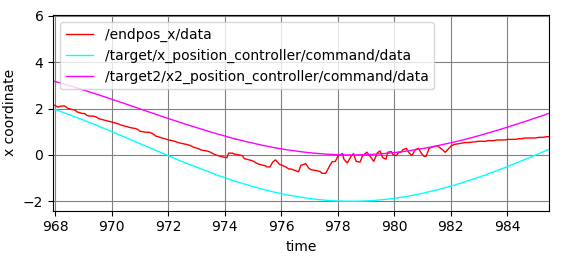
\includegraphics[width=\textwidth]{4.2.x.png}
    \caption{End effector x coordinate (/endpos/...) vs target sphere and box x coordinate (/target/...)}
  \end{minipage}
  \hfill
  \begin{minipage}[b]{0.44\textwidth}
    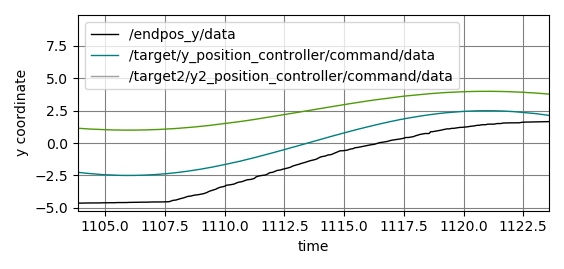
\includegraphics[width=\textwidth]{4.2.y.png}
    \caption{End effector y coordinate (/endpos/...) vs target sphere and box y coordinate (/target/...)}
  \end{minipage}
\begin{minipage}[b]{0.44\textwidth}
    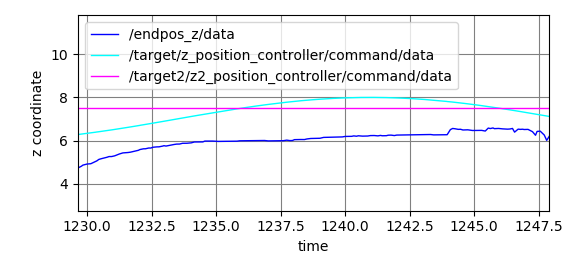
\includegraphics[width=\textwidth]{4.2.z.png}
    \caption{End effector z coordinate (/endpos/...) vs target sphere and box z coordinate (in world frame) (/target/...)}
  \end{minipage}
\end{figure}

\end{document}
